\chapter{EXPERIMENTAL RESULTS}
\label{chap:results}

This chapter reports the empirical results of the implemented Amazon Marketplace Intelligence Tracker. The purpose of the evaluation is not to prove a new machine-learning algorithm, but to assess whether the implemented data pipeline, analytics scripts, dashboard layer, and OpenClaw skill interface can produce useful competitive intelligence from real Amazon marketplace data. The chapter is organized into four parts: descriptive statistics of the collected dataset, evaluation of the sentiment and price-forecasting components, market intelligence findings, and operational observations from the deployed pilot.

\section{Data descriptive statistics}

The data collection window covered 13 calendar days, from April 17, 2026 to April 29, 2026. The system monitored three consumer-electronics categories: \textit{Gaming Keyboards}, \textit{True Wireless Earbuds}, and \textit{Portable Chargers}. The category-level ingestion job collected Top-50 ranking snapshots, while the watchlist ingestion job tracked detailed daily product snapshots for the thesis watchlist.

Across the observation window, the Supabase database contained 1,756 category ranking rows, 409 daily product snapshot rows, and 3,986 raw review records. These figures reflect the actual rows available after Apify extraction, parser normalization, and database upsert behavior; they are therefore reported as implementation outputs rather than idealized target counts. The latest cross-sectional category baseline, using the April 29, 2026 ranking snapshot, is summarized in Table~\ref{tab:category_baseline}.

\begin{table}[H]
  \centering
  \small
  \resizebox{\textwidth}{!}{%
  \begin{tabular}{l c c c c c c}
    \toprule
    \textbf{Category} & \textbf{ASINs} & \textbf{Mean Price} & \textbf{Price Range} & \textbf{Mean Stars} & \textbf{Mean Reviews} & \textbf{SOV} \\
    \midrule
    Gaming Keyboards        & 50 & \$65.31 & \$15.99 -- \$169.99 & 4.52 & 4,578  & 4.0\% \\
    True Wireless Earbuds   & 50 & \$86.61 & \$11.99 -- \$298.00 & 4.33 & 21,921 & 4.0\% \\
    Portable Chargers       & 50 & \$28.85 & \$12.34 -- \$199.99 & 4.48 & 6,949  & 4.0\% \\
    \bottomrule
  \end{tabular}}%
  \caption{Descriptive statistics of tracked categories on April 29, 2026. SOV denotes Sponsored Share of Voice, computed as the proportion of sponsored ASINs in the Top-50 snapshot. The uniform 4.0\% value across all three categories is a measurement artifact: the Apify actor flagged exactly two ASINs as sponsored in each Top-50 list ($2/50 = 4.0\%$), which likely under-counts true ad density because the actor captures only the labels visible on the first scrape pass.}
  \label{tab:category_baseline}
\end{table}

The three categories showed different competitive structures. True Wireless Earbuds had the highest mean price and the largest average review base, suggesting a more mature market with stronger incumbent review moats. Portable Chargers had the lowest mean price and a narrower mainstream pricing band, consistent with a more commoditized segment. Gaming Keyboards sat between the two, with a wider range of mid-priced and premium products.

\section{Empirical evaluation of analytical models}

Two model-based components were evaluated quantitatively: the RoBERTa sentiment classifier and the Prophet price forecaster. These evaluations use the repository outputs under \texttt{data/eval/} and should be interpreted as sanity checks for the deployed thesis prototype, not as large-scale benchmark studies.

\subsection{Sentiment classification}

The sentiment classifier was evaluated on $N = 3{,}851$ Amazon reviews using star ratings as a distant-supervision proxy: 1--2 stars were treated as negative, 3 stars as neutral, and 4--5 stars as positive. This proxy is imperfect because star ratings can reflect delivery, packaging, or expectation mismatch rather than textual sentiment alone, but it provides a reproducible evaluation target without manual labeling.

Two baselines were included to contextualise the result: VADER \citep{hutto2014vader}, a rule-based lexicon analyzer, and \texttt{nlptown/bert-base-multilingual-uncased-sentiment}, a BERT model fine-tuned directly on 1--5 star Amazon and Yelp reviews. The VADER compound score was thresholded at $\pm 0.05$ following the authors' convention. Table~\ref{tab:sentiment_baselines} reports the three-way comparison.

\begin{table}[H]
  \centering
  \begin{tabular}{lccccc}
    \toprule
    \textbf{Model} & \textbf{Accuracy} & \textbf{Macro $F_1$} & \textbf{Neg $F_1$} & \textbf{Neu $F_1$} & \textbf{Pos $F_1$} \\
    \midrule
    VADER (rule-based)      & 0.791 & 0.516 & 0.586 & 0.072 & 0.892 \\
    RoBERTa \emph{(deployed)} & 0.812 & 0.594 & 0.715 & 0.158 & 0.908 \\
    nlptown BERT            & \textbf{0.839} & \textbf{0.679} & \textbf{0.749} & \textbf{0.366} & \textbf{0.922} \\
    \bottomrule
  \end{tabular}
  \caption{Three-way sentiment model comparison against the star-rating proxy ($N = 3{,}851$). nlptown outperforms the deployed RoBERTa model on all metrics; see text for discussion.}
  \label{tab:sentiment_baselines}
\end{table}

Table~\ref{tab:sentiment_eval} reports the class-level breakdown for the deployed RoBERTa model.

\begin{table}[H]
  \centering
  \begin{tabular}{lccc}
    \toprule
    \textbf{Sentiment Class} & \textbf{Precision} & \textbf{Recall} & \textbf{\boldsymbol{$F_1$} Score} \\
    \midrule
    Negative (1--2 Stars) & 0.658 & 0.782 & 0.715 \\
    Neutral (3 Stars)    & 0.159 & 0.157 & 0.158 \\
    Positive (4--5 Stars) & 0.929 & 0.887 & 0.908 \\
    \midrule
    \textbf{Macro Average} & 0.582 & 0.609 & \textbf{0.594} \\
    \bottomrule
  \end{tabular}
  \caption{RoBERTa sentiment classification performance against a star-rating proxy.}
  \label{tab:sentiment_eval}
\end{table}

The evaluation reveals two patterns. First, RoBERTa outperforms the VADER lexicon baseline by 7.8 macro-$F_1$ points, confirming that contextual embeddings capture negation and mixed phrasing better than a rule-based lexicon. Second, nlptown achieves a higher macro-$F_1$ of 0.679, with a notably stronger neutral class ($F_1 = 0.366$ versus $0.158$). This gap has a structural explanation: nlptown was fine-tuned on product reviews rated on the same 1--5 star scale used as the evaluation proxy. Scoring against star-rating labels therefore partially measures how well each model predicts star ratings rather than latent review sentiment; nlptown benefits from this task alignment. RoBERTa, trained on Twitter data with a 3-class sentiment objective, is not optimised for star prediction and will be penalised by the proxy on borderline cases. The finding indicates that the proxy metric overestimates the relative gap between the two models on genuine sentiment classification. Replacing the deployed model with nlptown is a defensible direction for future work, though it would require re-running sentiment analysis on all stored reviews and re-evaluating downstream BMS and LQS outputs that depend on the sentiment score.

Figure~\ref{fig:sentiment_dist} summarizes the average positive, neutral, and negative review shares by category from the latest sentiment snapshot. The distribution is skewed toward positive reviews, especially in categories with mature products and large review bases. From an intelligence perspective, the most useful output is therefore not the positive majority itself, but the ability to isolate negative-review pockets and track them at ASIN level.

\begin{figure}[H]
  \centering
  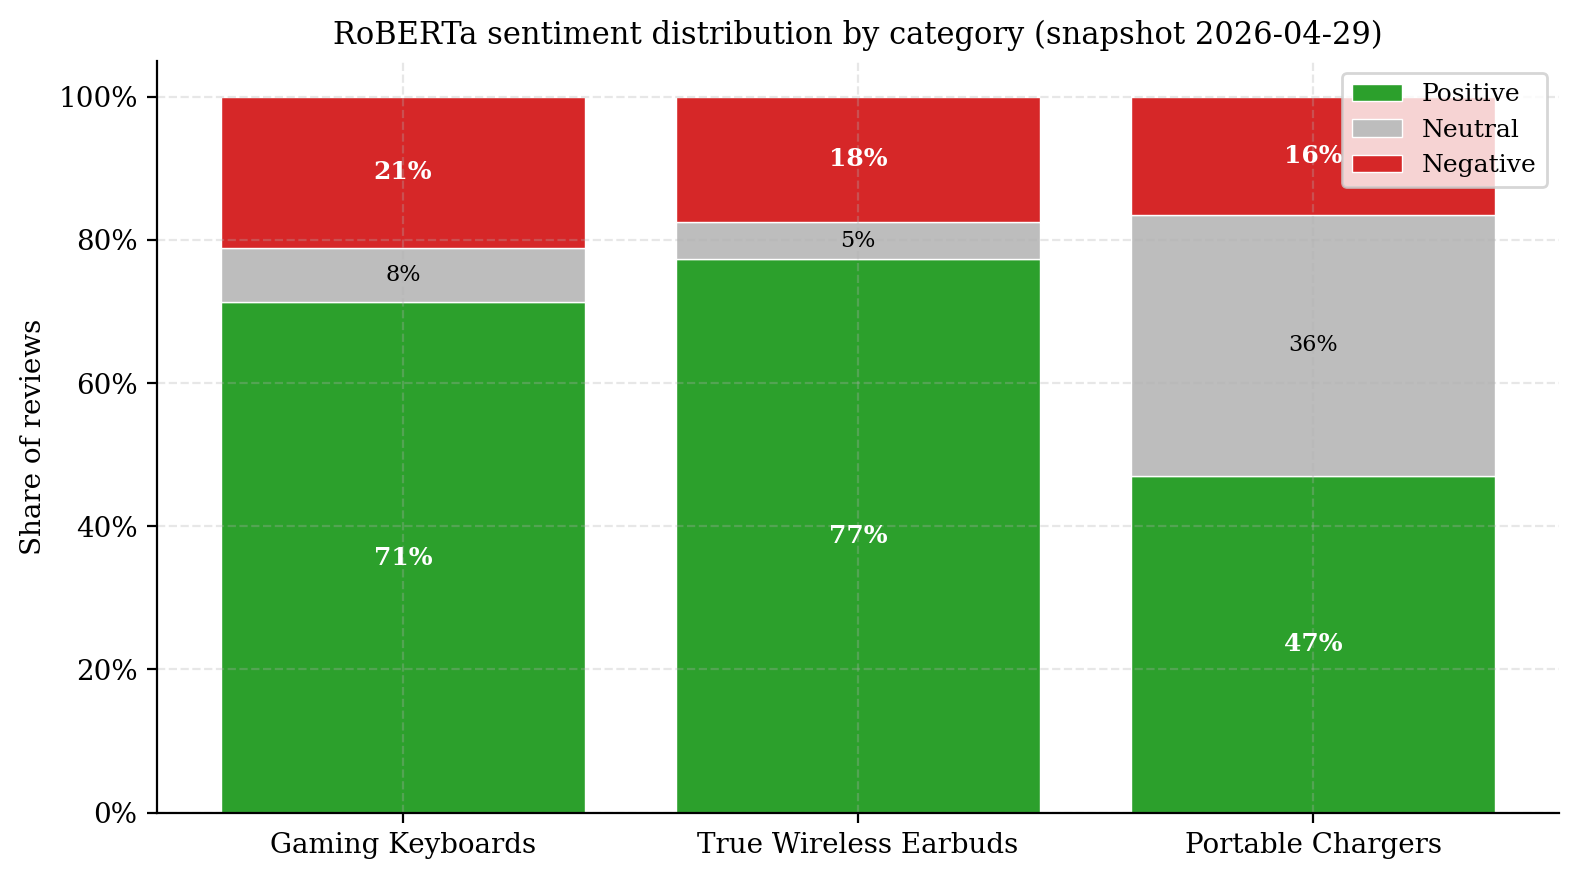
\includegraphics[width=0.85\textwidth]{figures/sentiment_distribution.png}
  \caption{Average RoBERTa sentiment composition by product category in the latest analysed review snapshot.}
  \label{fig:sentiment_dist}
\end{figure}

\subsection{Price-trend forecasting}

The price-forecasting component was evaluated using a five-way temporal holdout comparison. For each watchlist ASIN with sufficient price history, the final $H = 3$ observations were withheld, each candidate model was fitted on the earlier observations, and the resulting predictions were compared against the held-out prices using pooled Mean Absolute Error (MAE) and Mean Absolute Percentage Error (MAPE). The evaluation protocol required a minimum of $\texttt{MIN\_HISTORY} + H = 10$ price observations per ASIN, ensuring that each model had a viable training window.

\subsubsection*{Candidate models}

Five models were compared to identify the most suitable forecaster for short Amazon price series:

\begin{enumerate}
  \item \textbf{Naive (carry-forward)}: The last observed training price is repeated for all $H$ forecast steps. This baseline is deliberately simple; it performs well when prices are stationary.
  \item \textbf{Linear Trend (OLS)}: An ordinary least-squares regression is fitted on the training-window prices and extrapolated $H$ steps forward. This baseline captures monotonic drift.
  \item \textbf{Exponential Smoothing (ETS)}: Holt's additive trend model (no seasonality) is fitted via maximum-likelihood optimisation. ETS down-weights older observations exponentially, giving more influence to recent price movement.
  \item \textbf{ARIMA(1,1,0)}: A first-differenced autoregressive model of order one. First-differencing removes linear trend non-stationarity; the single AR lag allows the model to exploit serial autocorrelation in the differenced series.
  \item \textbf{Prophet}: Facebook Prophet with the \texttt{CMDSTANPY} backend, with daily, weekly, and yearly seasonality disabled. Prophet is retained in the deployed system because it additionally produces calibrated 80\% prediction intervals (\texttt{yhat\_lower}, \texttt{yhat\_upper}), which the Momentum Strategist agent exposes as volatility signals.
\end{enumerate}

For models experiencing convergence failure on individual ASINs (a risk with ARIMA and ETS on very flat series), the implementation falls back to the naive prediction for that ASIN, and the failure is logged as a warning. This occurred on a small subset of ASINs and did not affect the pooled result materially.

\subsubsection*{Results}

All 30 watchlist ASINs met the minimum history threshold of 10 observations. Table~\ref{tab:forecast_comparison} reports the pooled MAE ranking across all five methods.

\begin{table}[H]
  \centering
  \begin{tabular}{lcc}
    \toprule
    \textbf{Model} & \textbf{Pooled MAE (\$)} & \textbf{Rank} \\
    \midrule
    Naive (carry-forward)    & 1.292 & 1\textsuperscript{st} \\
    ARIMA(1,1,0)             & 1.323 & 2\textsuperscript{nd} \\
    ETS (Holt additive)      & 2.324 & 3\textsuperscript{rd} \\
    Linear Trend (OLS)       & 2.906 & 4\textsuperscript{th} \\
    Prophet \emph{(deployed)} & 2.970 & 5\textsuperscript{th} \\
    \bottomrule
  \end{tabular}
  \caption{Five-way price forecast comparison on 30 watchlist ASINs ($H = 3$ days, $N_{\min} = 10$ training observations). Pooled MAE is computed over all held-out price points across all evaluated ASINs. Lower is better.}
  \label{tab:forecast_comparison}
\end{table}

The naive carry-forward baseline achieves the lowest pooled MAE of \$1.292. ARIMA(1,1,0) is the closest competitor at \$1.323 — only 2.4\% higher than naive — while ETS, Linear Trend, and Prophet trail by wider margins. Prophet's pooled MAPE was 6.75\%, and the empirical coverage of its 80\% prediction intervals was 67.8\%, below the nominal 80\% target.

\subsubsection*{Interpretation}

The dominance of the naive baseline across all more complex alternatives is a well-documented property of short, near-stationary price series \citep{makridakis2018m4}. Amazon marketplace prices are frequently held constant for days or weeks; in such conditions, carry-forward trivially minimises expected absolute error, and any model that attempts to learn trend or autocorrelation risks introducing estimation noise that exceeds its signal gain. The near-equivalence of ARIMA and naive (MAE gap of \$0.031) further supports the interpretation that the observed price series approximates a random walk over short horizons: the differenced AR(1) structure captures essentially no additional predictable autocorrelation beyond what carry-forward already exploits.

The underperformance of ETS, Trend, and Prophet relative to naive is consistent with overfitting on a training window of approximately 7--12 observations: each model has sufficient parameters to learn the specific trajectory of the training prices rather than the underlying generating process. This is an inherent data-volume constraint rather than a deficiency in the models themselves.

\subsubsection*{Model selection for deployment}

Despite ranking fifth on point-forecast MAE, Prophet is retained as the production forecasting model for two reasons. First, it is the only evaluated model that produces calibrated probabilistic prediction intervals (\texttt{yhat\_lower}, \texttt{yhat\_upper}), which the Momentum Strategist agent uses to signal short-term price volatility rather than a precise point estimate. No equivalent uncertainty envelope is natively available from the ARIMA or Naive implementations used here. Second, Prophet's accuracy disadvantage is expected to diminish as data accumulates: with 30 or more observations per ASIN, the model's changepoint detection and trend-fitting become more reliable. The thesis system is designed as a continuous pipeline, so forecast quality should improve organically over time without requiring code changes.

In summary, the evaluation confirms that price forecasting is currently a \emph{directional and volatility signal} rather than a precise prediction engine. This finding is disclosed to end-users through the agent system prompt and is a documented limitation of the prototype.

\section{Market intelligence findings}

The analytics scripts produced several interpretable competitive signals: entrant and exit events, price-tier segmentation, listing quality scores, brand momentum scores, alert records, and image-change flags. The following subsections summarize the most important findings from the observation window.

\subsection{Competitive entrances and exits}

The Top-50 ranking monitor recorded 1,060 entrant and exit events across the three categories: 528 entrant events and 532 exit events. Because the measurement boundary is a Top-50 list, these two counts are expected to be similar over time; products entering the observed set usually imply that other products leave it.

Portable Chargers had the highest churn, with 204 entrant events and 201 exit events. Gaming Keyboards recorded 171 entrants and 183 exits, while True Wireless Earbuds recorded 153 entrants and 148 exits. The higher churn in Portable Chargers suggests a more fluid competitive environment, likely shaped by dense pricing competition and frequent promotional movement.

\begin{figure}[H]
  \centering
  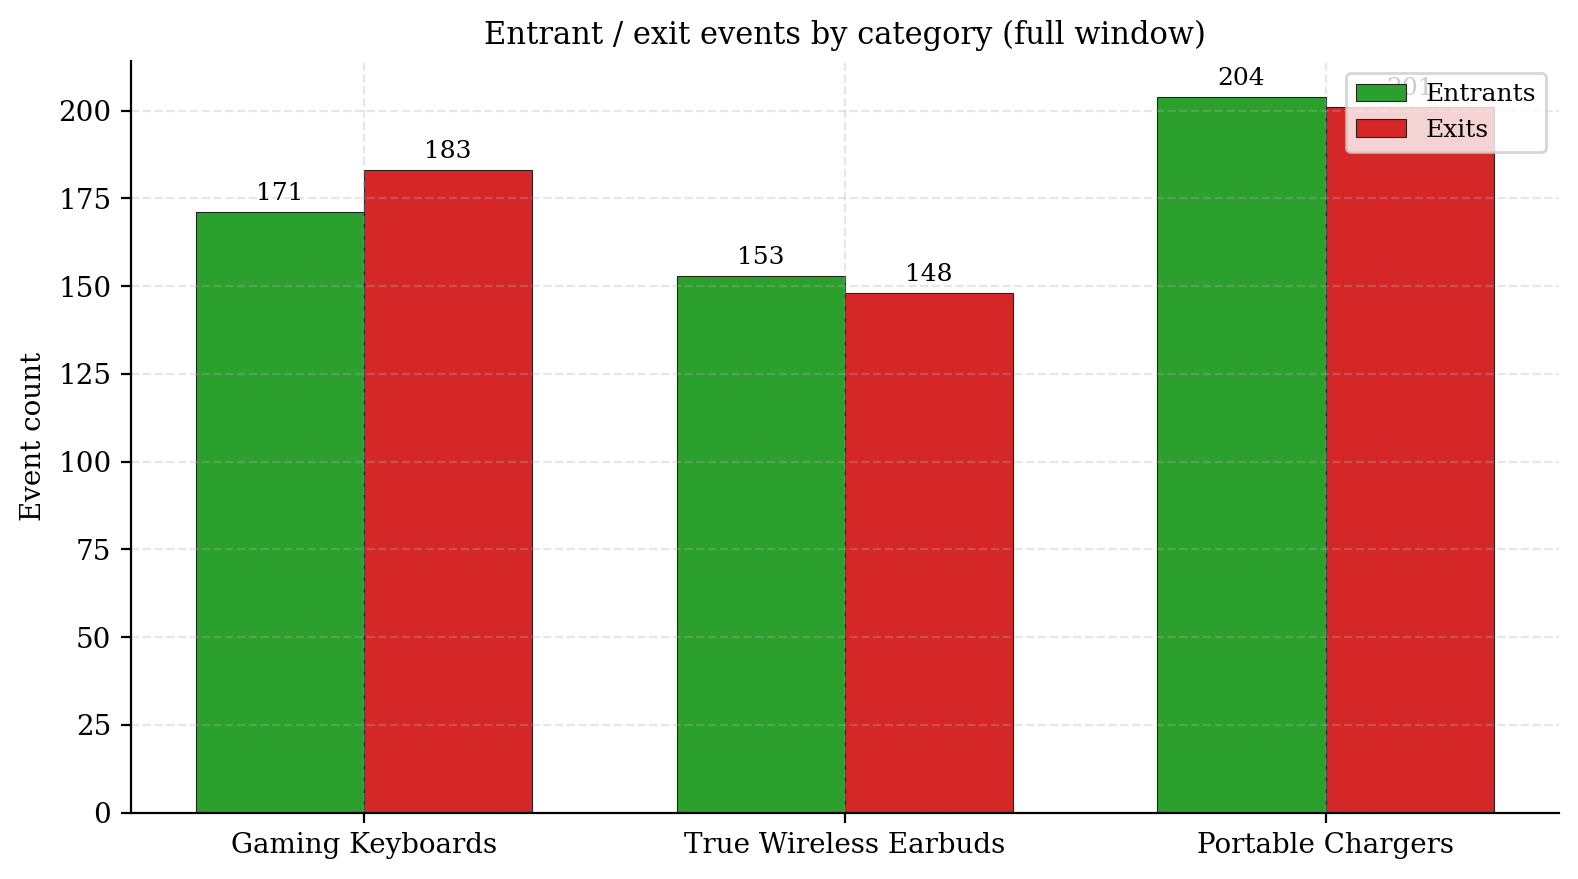
\includegraphics[width=0.85\textwidth]{figures/entrant_exit_by_category.png}
  \caption{Top-50 entrant and exit events by product category over the 13-day observation window.}
  \label{fig:entrant_exit}
\end{figure}

\subsection{Price tier segmentation}

The price-tier pipeline used K-Means clustering with $k=3$ to assign available priced ASIN records into entry, mid-range, and premium tiers within each category. This dynamic approach avoids hard-coded price thresholds, which would not transfer well between low-price categories such as Portable Chargers and higher-price categories such as True Wireless Earbuds. The code uses $k = \min(3, \text{number of unique prices})$, so on days with fewer than three distinct price points the algorithm collapses to fewer clusters; all records are assigned to the entry tier if only one unique price exists. This fallback is logged but is not expected to affect the majority of daily snapshots in a Top-50 list.

For True Wireless Earbuds, the latest tier table assigned 39 ASIN records to the entry tier with a mean price of \$28.04, 16 to the mid-range tier with a mean price of \$101.10, and 12 to the premium tier with a mean price of \$230.66. These are priced ASIN records across ranking snapshots rather than a count of unique products, so the total can exceed the Top-50 category size when an ASIN appears on multiple collection days. The tier labels therefore provide a more context-aware comparison basis for dashboards and agent summaries than a single category-wide average price.

\begin{figure}[H]
  \centering
  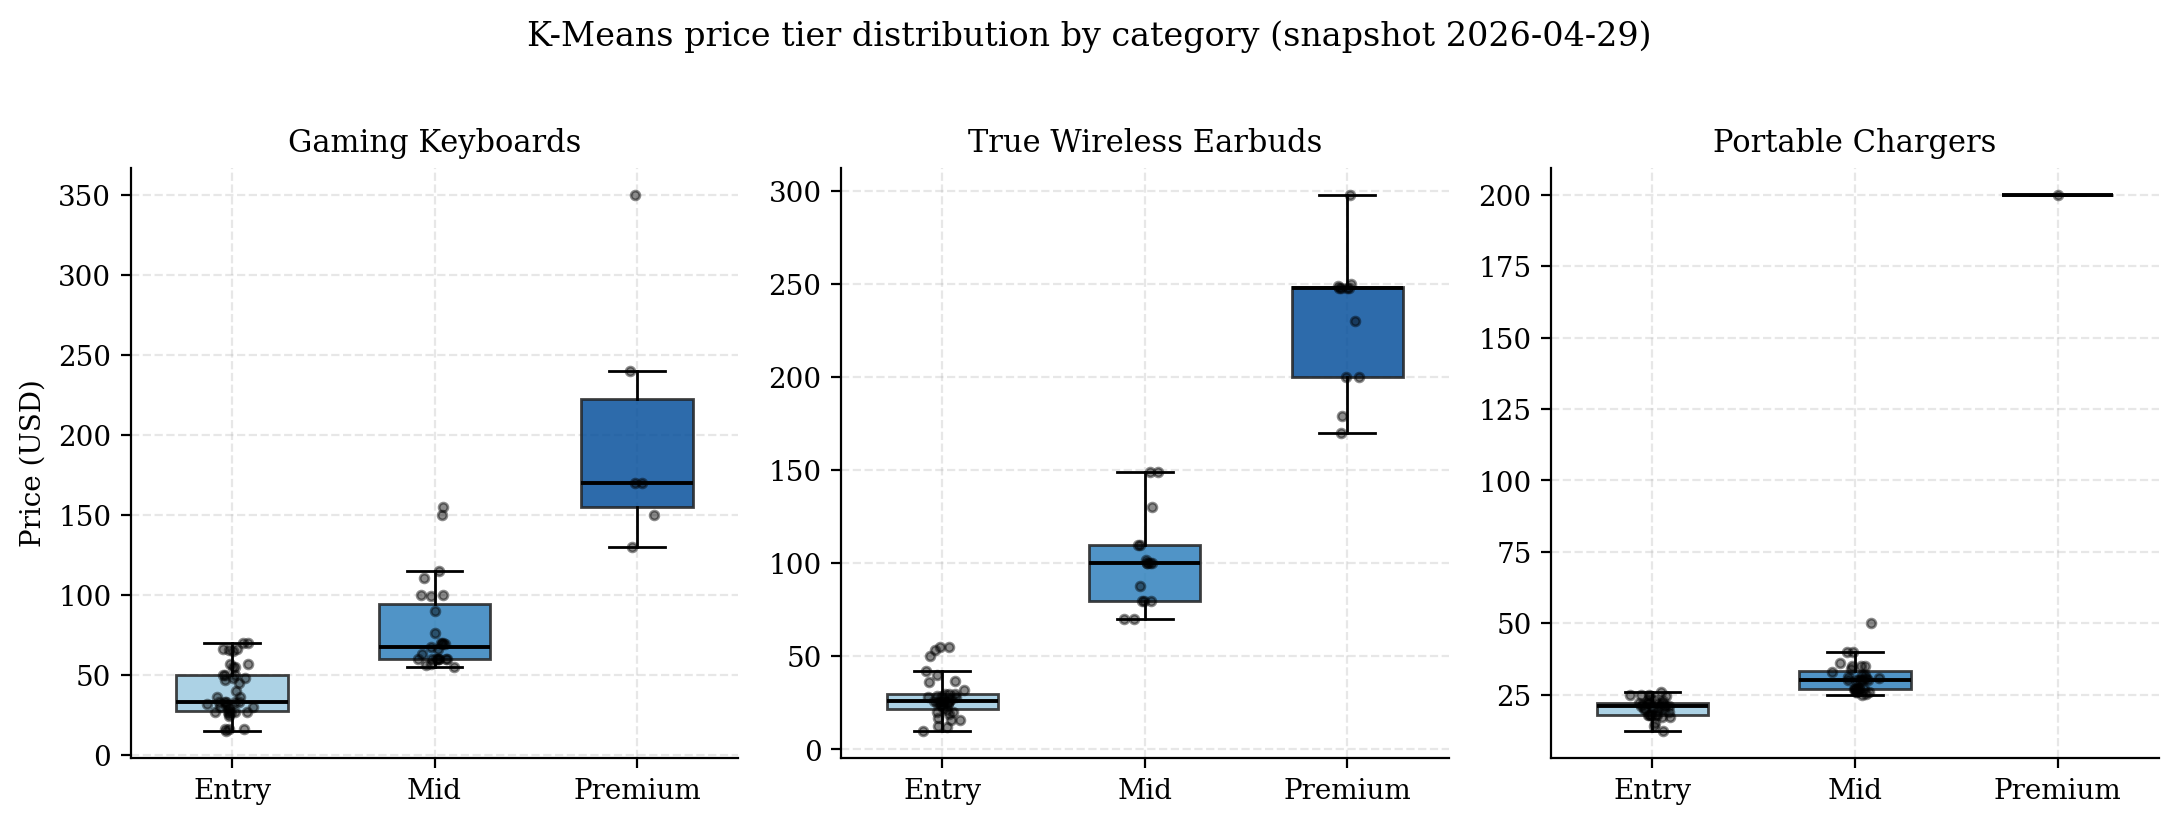
\includegraphics[width=0.85\textwidth]{figures/price_tier_distribution.png}
  \caption{K-Means price tier distribution by category, showing entry, mid-range, and premium clusters.}
  \label{fig:price_tier}
\end{figure}

\subsection{Listing quality and brand momentum}

The Listing Quality Score (LQS) was computed for 30 watchlist ASINs. Scores were high overall, with a mean of 93.4, a median of 94.2, a minimum of 79.5, and a maximum of 96.9. Gaming Keyboards had the highest average LQS at 95.5, followed by Portable Chargers at 93.1 and True Wireless Earbuds at 91.5. The top ASIN was B0C9ZJHQHM with an LQS of 96.9.

This result suggests that basic listing hygiene is already strong among the tracked products. In such a saturated listing environment, the LQS is most useful for identifying weak outliers rather than explaining all ranking movement. For example, the lowest observed score was B0FQFB8FMG at 79.5, which would be a clearer candidate for listing-page improvement than products already scoring above 95.

\begin{figure}[H]
  \centering
  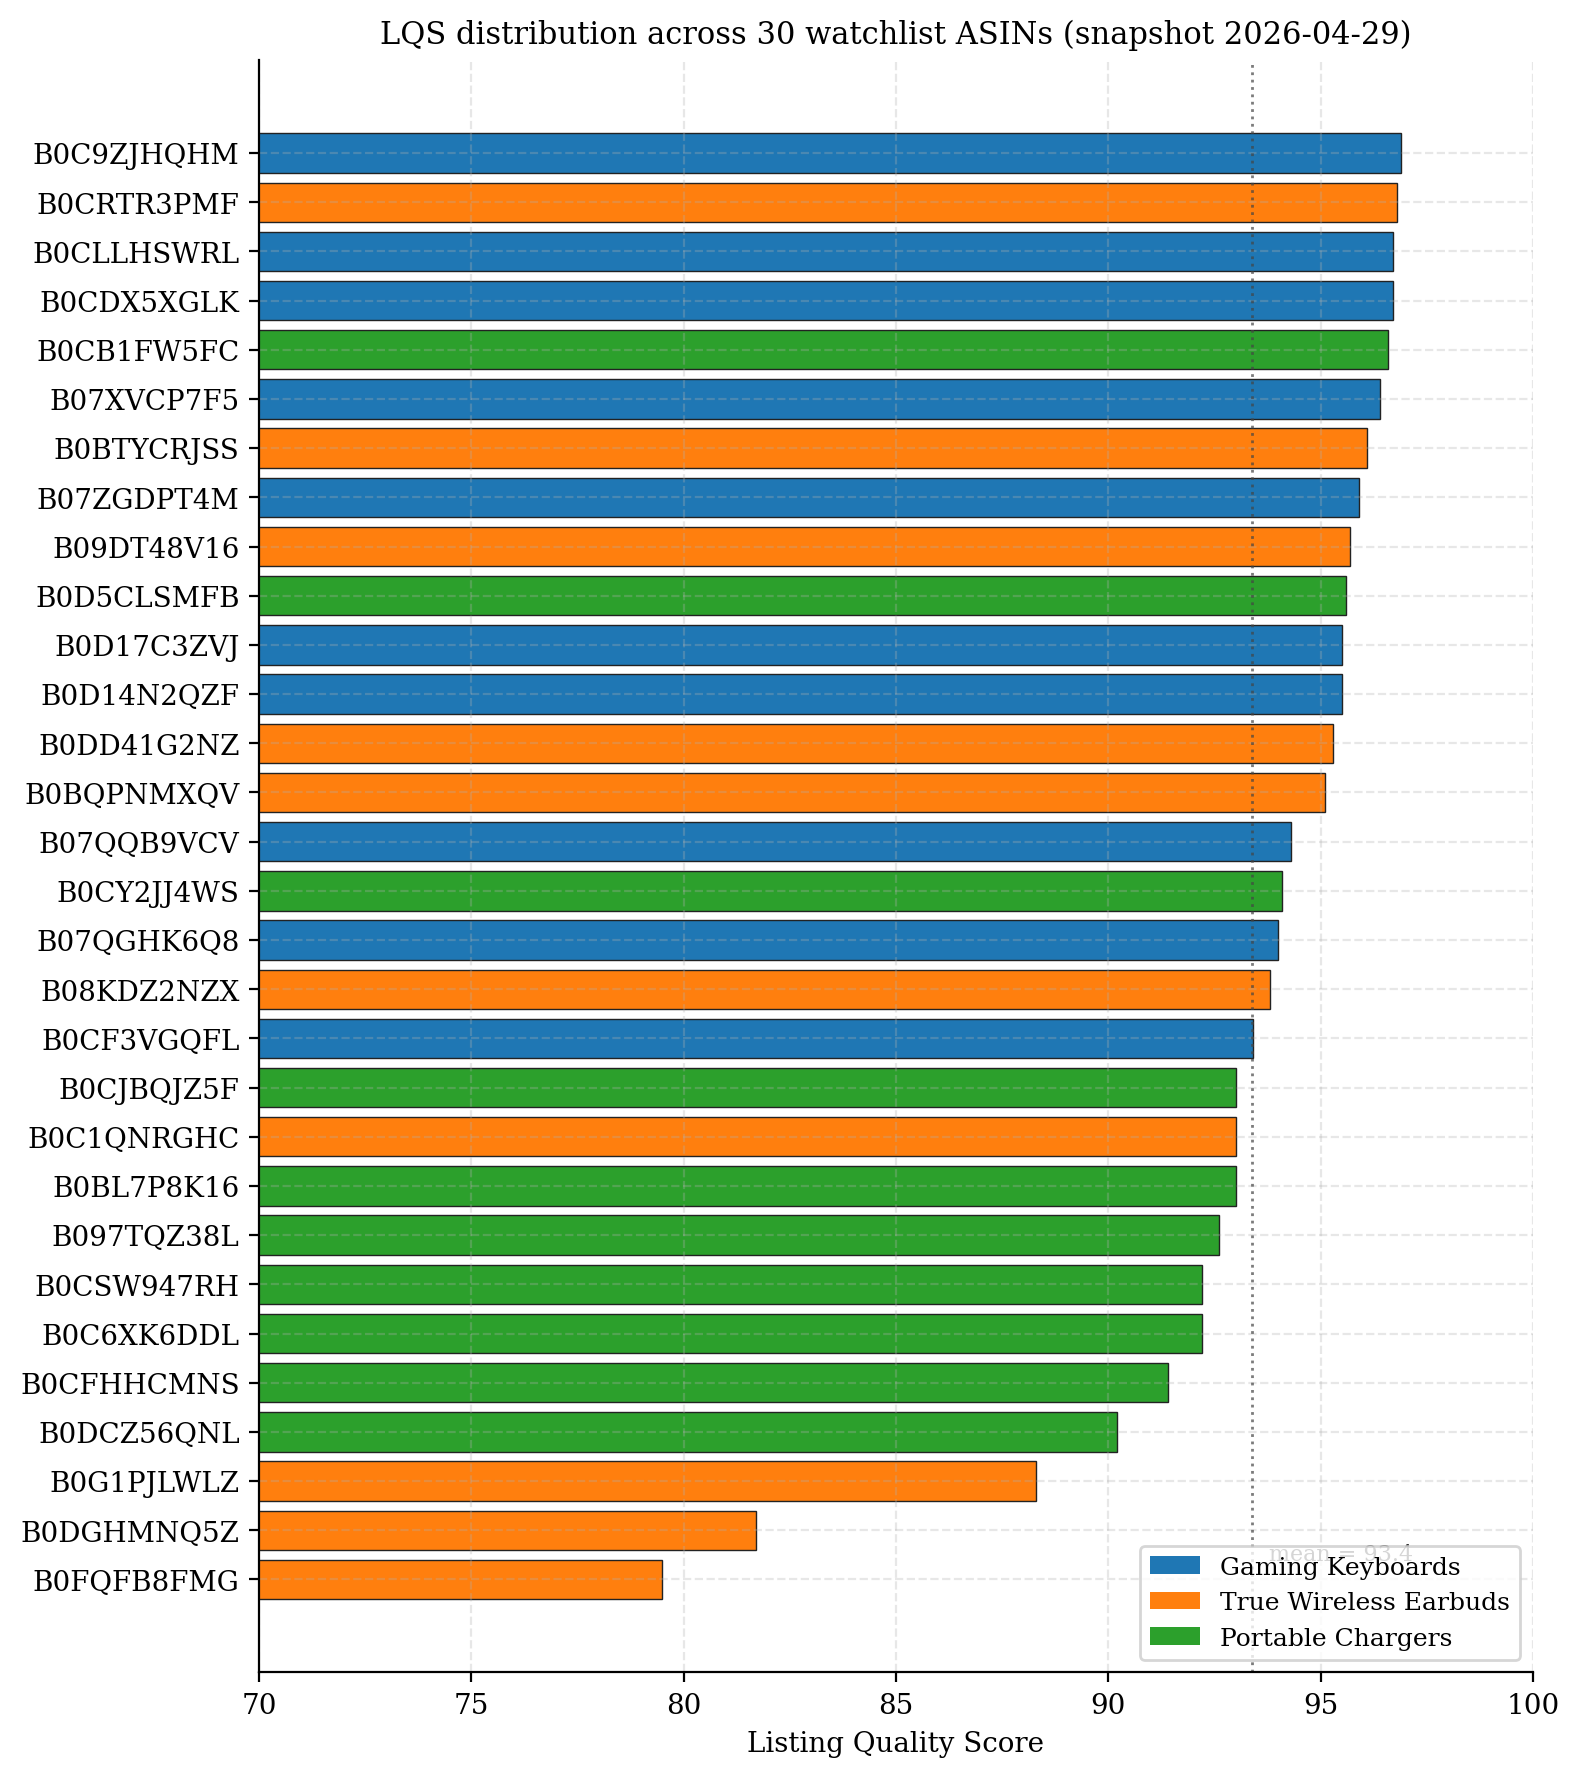
\includegraphics[width=0.85\textwidth]{figures/lqs_distribution.png}
  \caption{Distribution of Listing Quality Scores across the 30 watchlist ASINs.}
  \label{fig:lqs_dist}
\end{figure}

The Brand Momentum Score (BMS) ranked products by combining normalized BSR movement, review velocity, and sentiment score. The highest momentum ASIN in the latest output was B0CB1FW5FC in Portable Chargers, with a BMS of 0.752, review velocity of 116 reviews, and sentiment score of 0.710. Other high-scoring ASINs included B0CRTR3PMF and B09DT48V16 in True Wireless Earbuds. These outputs are useful because they turn separate raw signals into a concise shortlist for competitor monitoring.

\begin{figure}[H]
  \centering
  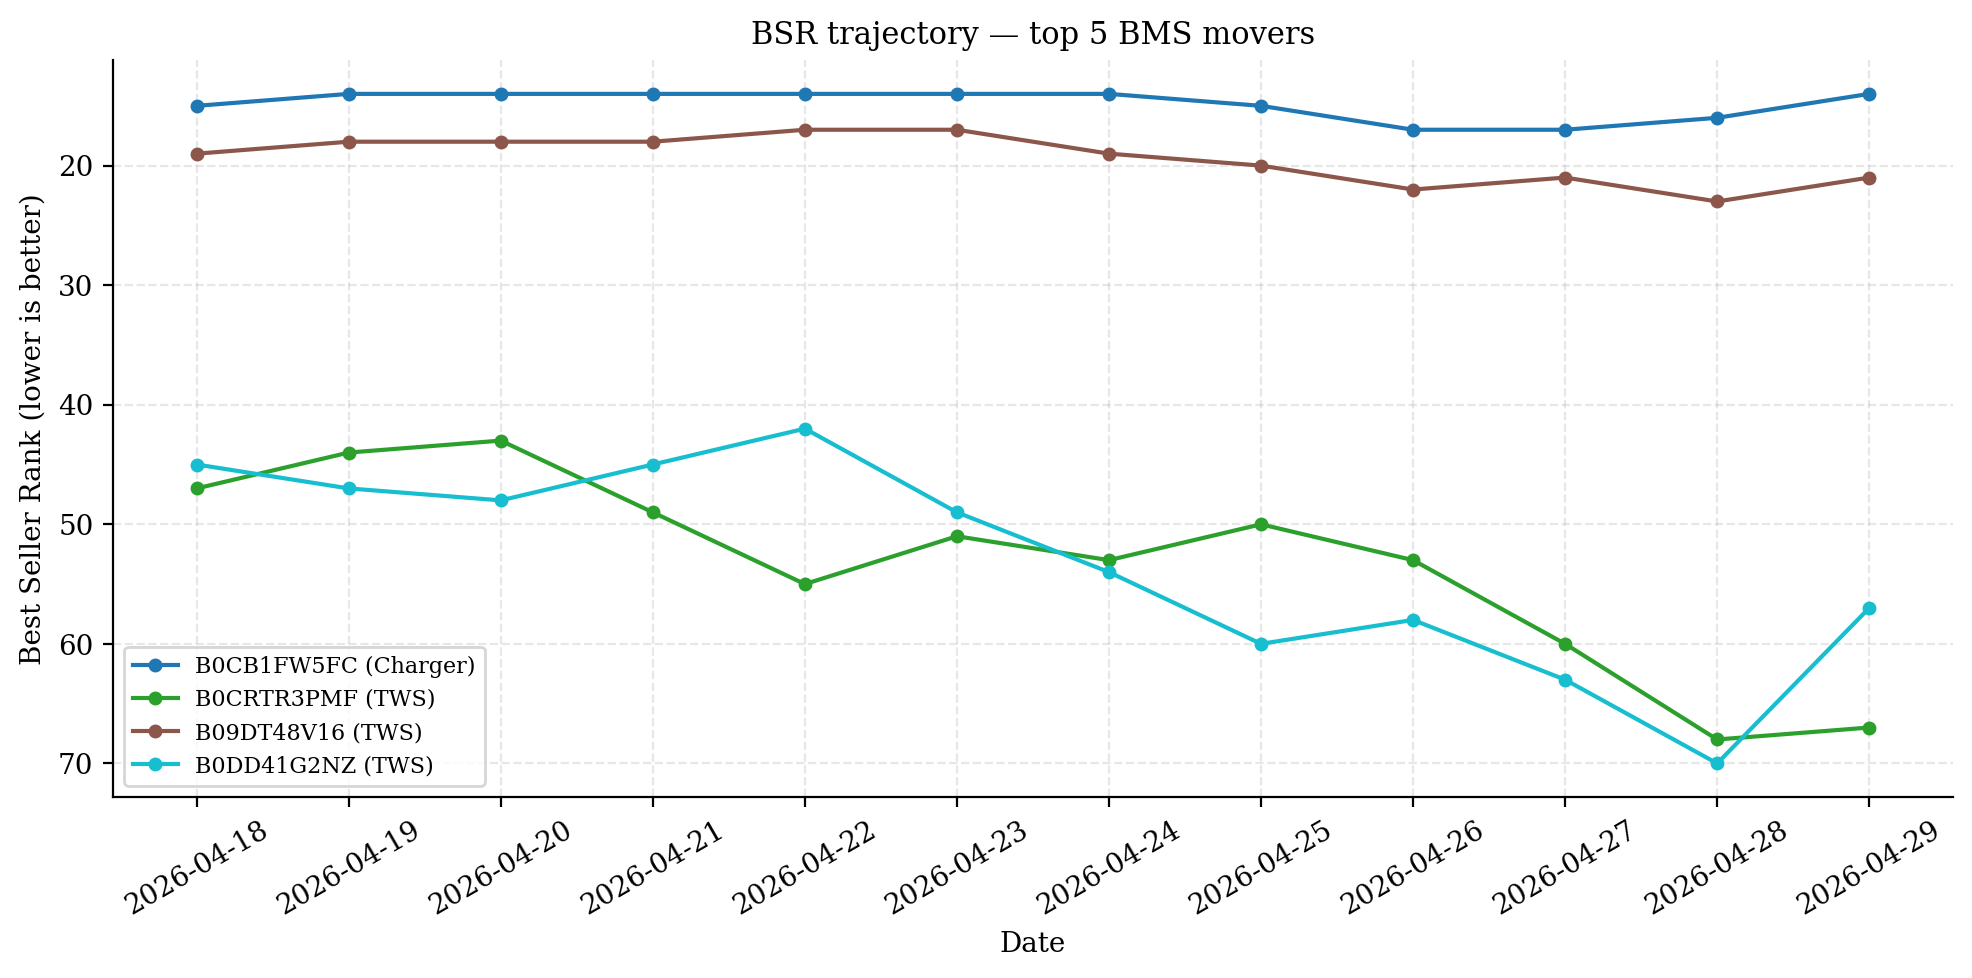
\includegraphics[width=0.85\textwidth]{figures/bsr_trend.png}
  \caption{Best Seller Rank trajectories for the top five BMS movers. Lower BSR values indicate better sales rank.}
  \label{fig:bsr_trend}
\end{figure}

\subsection{Image-change detection}

The image-change pipeline used perceptual hashing to compare product image snapshots. During the observed window, no actual image-change event exceeded the configured pHash threshold. This is a useful negative result: the system had the mechanism to detect stealth listing-image redesigns, but the tracked window did not contain a qualifying change. Therefore, the thesis should treat image-change detection as an implemented monitoring capability rather than as an empirically frequent event in this dataset.

\section{Operational performance of the intelligence layer}

The operational layer converts the analytics tables into dashboard views and Telegram-facing agent responses. The relevant evaluation question is whether the generated data is structured enough for the Streamlit/web dashboards and the OpenClaw read-only skills to consume consistently.

\subsection{Alert generation}

The rule-based alert engine generated 1,248 alert records across the observation window. The alert table contained 593 \texttt{new\_entrant} alerts, 648 \texttt{exit} alerts, 6 \texttt{price\_drop} alerts, and 1 \texttt{stockout} alert. By severity, the distribution was 542 low-severity alerts, 651 medium-severity alerts, and 55 high-severity alerts.

\begin{figure}[H]
  \centering
  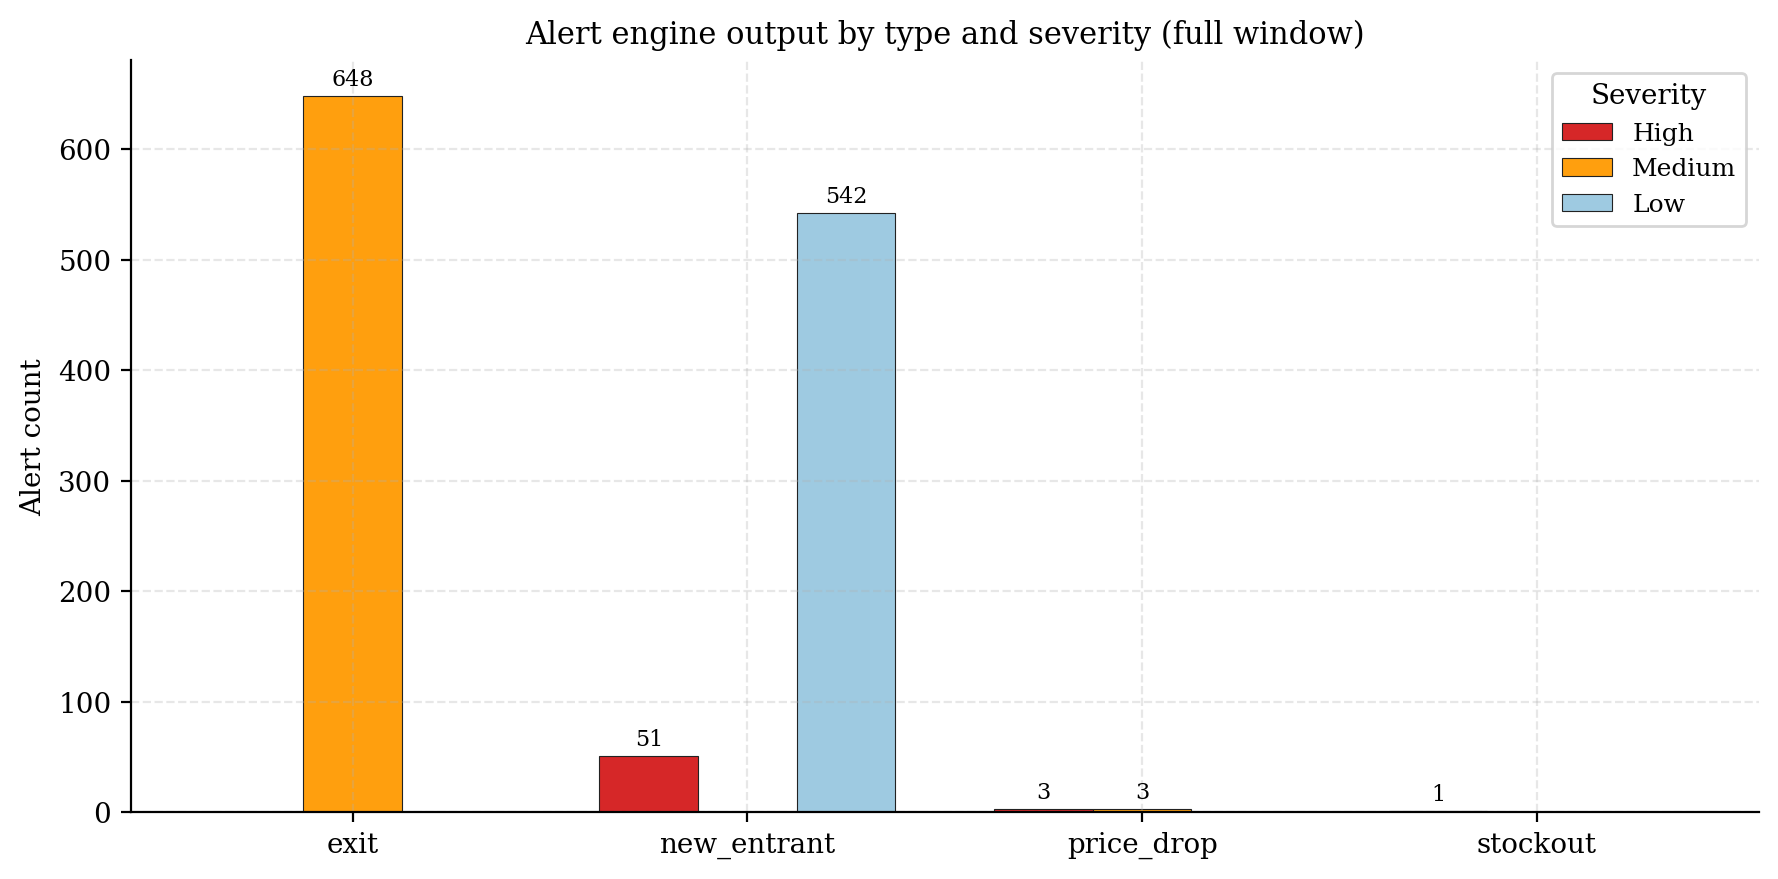
\includegraphics[width=0.85\textwidth]{figures/alerts_breakdown.png}
  \caption{Alert engine output by alert type and severity over the observation window.}
  \label{fig:alerts_breakdown}
\end{figure}

The alert distribution is consistent with the intended design. Routine Top-50 exits and non-top-10 entrants create most of the operational volume, while price drops, stockouts, and top-10 entrants form a smaller high-priority subset. This structure helps the Momentum Strategist agent focus on a manageable number of urgent events instead of forwarding every market movement with equal weight.

\subsection{Dashboard and agent consumption}

The same Supabase-derived tables supported both pull-based and push-based consumption. The Streamlit dashboard and public web dashboard provide analyst-controlled exploration, while the OpenClaw agents consume the data through 13 read-only Python skills. This separation is important: analytics scripts and scheduled jobs write to Supabase, but agent skills only read and summarize existing records. The resulting architecture reduces the risk of accidental database mutation through conversational interfaces.

The three Telegram-bound agents also map cleanly to the analytical outputs. Competitor Spy uses ranking, BMS, entrant/exit, sponsored-share, price-tier, and image-change skills. Sentiment Detective uses sentiment, review, aspect, and snapshot skills. Momentum Strategist uses alerts, BMS, price forecast, LQS, and sentiment skills. The pilot therefore demonstrates that the same analytics backbone can support multiple specialized decision views without duplicating data pipelines.

\subsection{Cost profile}

The deployed pilot remained inexpensive because most computation ran through scheduled Python jobs and free or low-cost managed services. Supabase stored the operational tables, GitHub Actions handled scheduled orchestration, and OpenClaw handled the Telegram agent layer. The main recurring cost during the pilot was Apify usage for Amazon data extraction, estimated at approximately \$8--\$10 per month for the thesis-scale workload. Generative AI usage through \texttt{gpt-5.4-mini} was below \$1 for the tested interaction volume. At this scale, the total monthly operating cost was therefore approximately \$11 or less, making the framework realistic for a student project or small-market monitoring pilot.
